\begin{frame}
\frametitle{Introduction}
Several applications in statistics lead to large and dense matrices:
\begin{itemize}
\item Karhunen-Loève decomposition;
\item Kriging;
\item applications using large covariance matrices (ex: random Gaussian sampling).
\end{itemize}

\begin{block}{Covariance matrices}
Let $Z:\mathbb{R}^d \mapsto \mathbb{R}$ be some random process, stationnary of 
order 2. We have N observation points $\left\{ x_i \in \mathbb{R}^d /i=1,\hdots,N \right\}$ with values $Z(x_i)$.
Let assume that the covariance of these points is known and given by a matrix $K \in \mathbb{R}^{N \times N}$ with

\[ K_{ij} = \mathrm{Cov}(Z(x_i),Z(x_j)) \]
%\begin{itemize}
%\item Symetric Positive Definite (SPD) matrix;
%\item Many solves;
%\item Usually,
% \begin{itemize}
%  \item Cholesky decomposition $K=LL^T$;
%  \item Forward/Backward substitutions.
% \end{itemize}
%\end{itemize}
\end{block}
\end{frame}

%\begin{frame}
%\frametitle{Covariance matrices}
%\framesubtitle{}
%
%Let $Z:\mathbb{R}^d \mapsto \mathbb{R}$ be some random process, stationnary of 
%order 2. We have N observation points $\left\{ x_i \in \mathbb{R}^d /i=1,\hdots,N \right\}$ with values $Z(x_i)$.
%Let assume that the covariance of these points is known and given by a matrix $K \in \mathbb{R}^{N \times N}$ with
%
%\[ K_{ij} = \mathrm{Cov}(Z(x_i),Z(x_j)) \]
%
%\end{frame}

\begin{frame}
\frametitle{Covariance matrices}
\framesubtitle{covariance kernel}

%Consider a covariance matrix $K$.
\begin{itemize}
  %\item $K$ is SPD (covariance matrix);
  \item usually $K$ is not known exactly:
    \begin{itemize}
    \item modelled as a convolution matrix of a kernel $k: \mathbb{R}^d \mapsto \mathbb{R}_{\plus}$:
       \[ K_{ij} := k(x_i,x_j) \]
    \item what is $k$?
    \begin{itemize}
      \item Exponential:
       \[ k(x,y) = e^{-|x-y|/\lambda} \]
      \item Gaussian:
       \[ k(x,y) = e^{-|x-y|^2/(2\lambda^2)} \]
      \item Quadratic:
       \[ k(x,y) = \left(1+\frac{|x-y|}{2 \lambda} \right)^{-2}  \]
      \item and many more!
    \end{itemize}
 \end{itemize}

  \item N can be large. For instance, every node in a FEM discretization;
\end{itemize}
\end{frame}

\begin{frame}
\frametitle{Covariance matrices}
\framesubtitle{linear algebra}
\begin{itemize}
\item K is ill-conditionned, many RHS: direct solver;
\item K is SPD: Cholesky.
\end{itemize}

\begin{block}{Complexity (LAPACK)}
  \begin{itemize}
    \item Cholesky factorization (DPOTRF): $1/3N^3 + 1/2N^2 + 1/6N$
    \item Solving (DPOTRS): $N_{\mathrm{RHS}} \times 2N^2$
    \item Storage: $8N^2/2$
  \end{itemize}
\end{block}
\alert{Need of a fast direct solver: \hmat framework.}
\end{frame}

\begin{frame}
\frametitle{Toy model: exponential kernel in 1D}
Let $X_N$ be a uniform discretization of $[0,1]$ with the 
discretization step $h = \frac{1}{N-1}$ : 

\[ X_N = \left\{ 0=x_1,\hdots,x_N=1\right\} 
\]

The correlation length $\lambda$ is set to $\lambda:=5h$ and the exponential kernel in 1D reads as 

\[ K_{\lambda}(x_i,x_j) = e^{-|x_i-x_j|/\lambda} 
\]
\end{frame}


\begin{frame}
\frametitle{Toy model: exponential kernel in 1D}
\only<1|handout:4>{
\begin{figure}
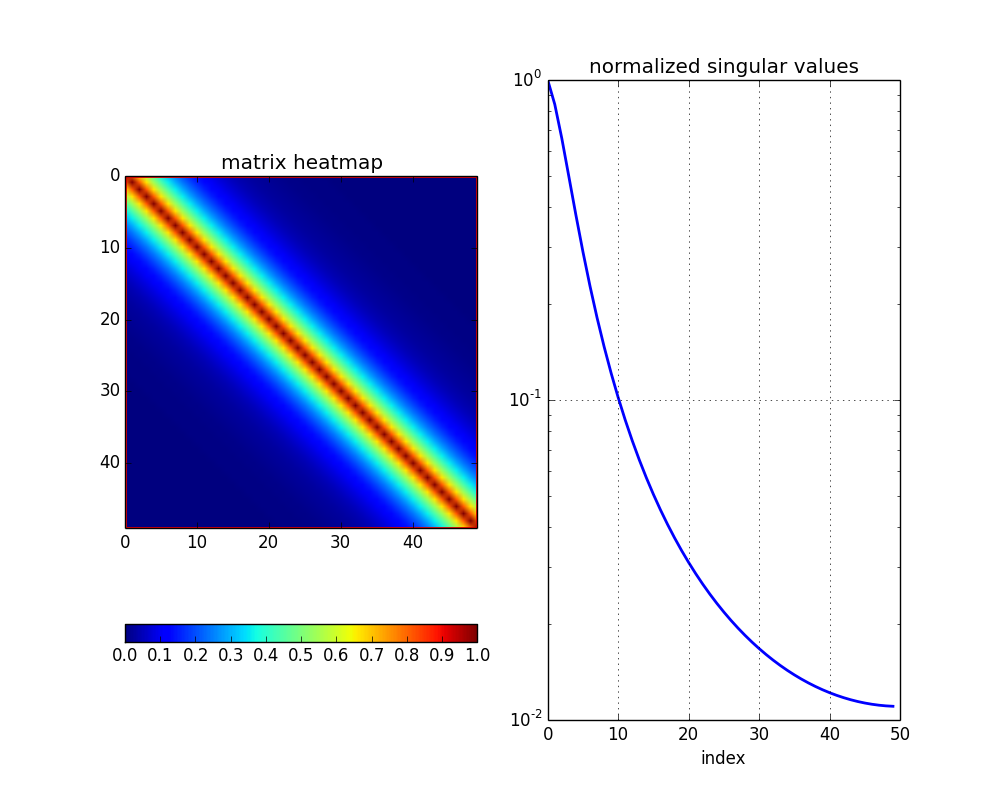
\includegraphics[scale=0.3]{./img/original_matrix_exp_1d.png}
\caption{the covariance matrix $K_{\lambda}([0,1],[0,1])$}
\end{figure}
}
\only<2|handout:4>{
\begin{figure}
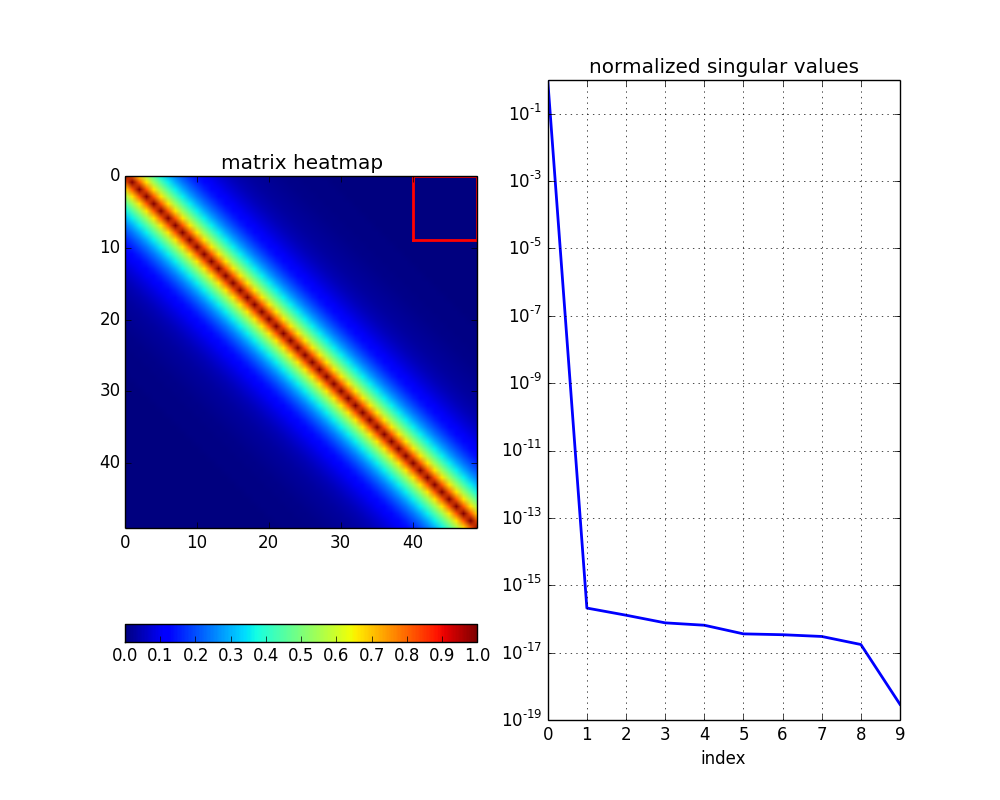
\includegraphics[scale=0.3]{./img/original_matrix_exp_1d_small.png}
\caption{small extra-diagonal block: $K_{\lambda}([0,0.2],[0.8,1])$ }
\end{figure}
}
\only<3|handout:4>{
\begin{figure}
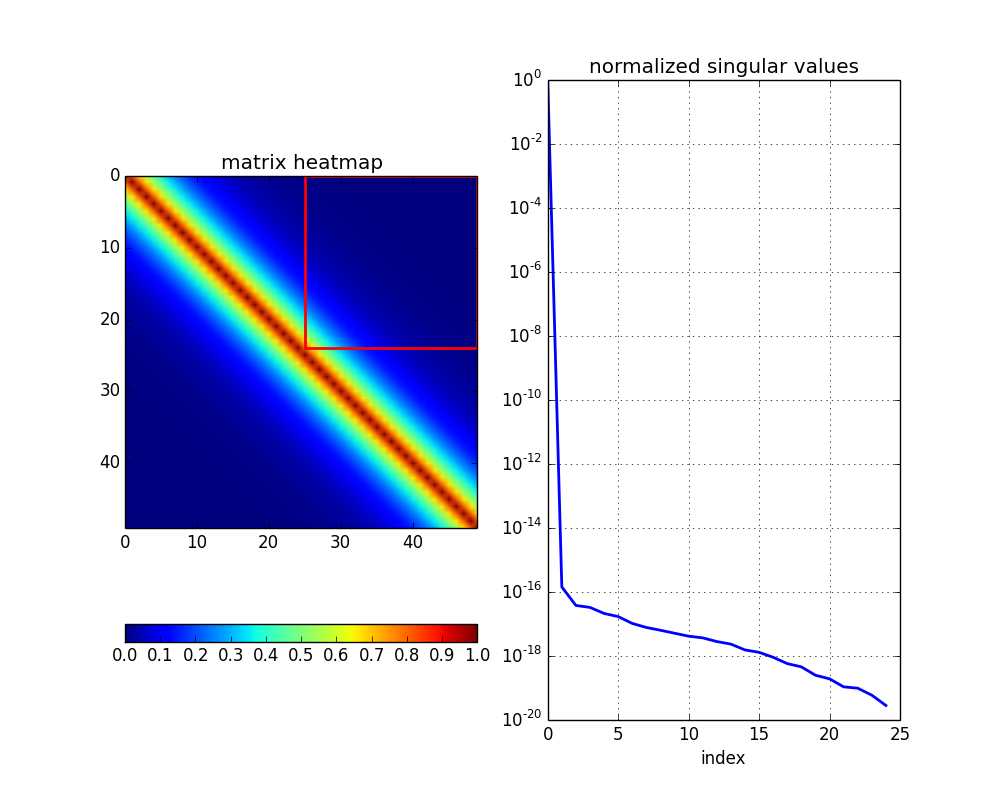
\includegraphics[scale=0.3]{./img/original_matrix_exp_1d_big.png}
\caption{large extra-diagonal block: $K_{\lambda}([0,0.5],[0.5,1])$ }
\end{figure}
}
\only<4|handout:4>{
\begin{figure}
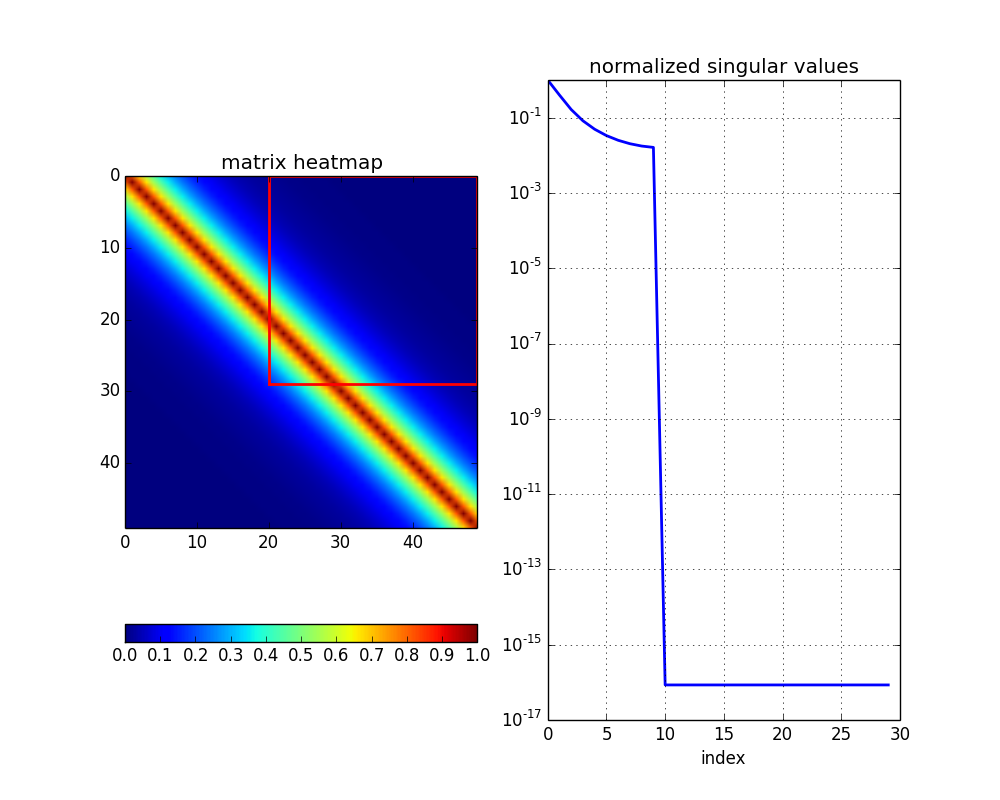
\includegraphics[scale=0.3]{./img/original_matrix_exp_1d_diag.png}
\caption{taking a part of the diagonal: $K_{\lambda}([0,0.6],[0.4,1])$ }
\end{figure}
}
\end{frame}

\begin{frame}
\frametitle{Toy model: exponential kernel in 1D}
Whenever $x_i$ and $x_j$ are in disjoint sets the kernel reads as a separated one. For instance; if $x_i > x_j$ then 

\[ K_{\lambda}(x_i,x_j) = e^{(x_j-x_i)/\lambda} = e^{x_j/\sqrt{\lambda}}e^{-x_i/\sqrt{\lambda}} , 
\]
which is of rank 1.
\end{frame}

